% !TEX root = ../main.tex


\chapter{Approach}
%TODO:
% was erwartet mich in diesem kaitel
% warum bin ich so vorgegangen
% was wird am ende stehen (ohne genaue werte)
% wo können referenzen gefunden werden? http://www.cplusplus.com

\section{Switching The Synchronization}
The first step taken was switching from the pthread library to a compare and swap (CAS) algorithm. Since C++ 11 there is an equivalent implementation in the standard library called \inline{bool std::atomic::compare\_exchange\_weak(T\& expected, T val)} (or \inline{bool std::atomic::compare\_exchange\_strong(T\& expected, T val)}) that was used for this task. This function compares the current value of an \inline{std::atomic} with \inline{expected} and replace it with \inline{val} if the comparison returns true. If it returns false it replaces \inline{expected} with the actual value of the atomic. The weak version is allowed to return false in favor for a general performance gain, even if the compared values are actually equal.

To represent a lock that can either be locked or unlocked, a boolean as value is sufficient. To shape a spin lock like mutexes and semaphores with a CAS function, they have to loop until the expected value compares equal. There are two reasonable modes to lock: the first is to just wait until an observed lock is unlocked and the second is to wait for an unlock with an immediate locking. The first approach can be helpful to suspend the execution of the current thread until an external thread is signalling a continuation. The second approach can be used to block access to a resource until all preceeding manipulations are completed. At last there are functions necessary that can block or release the resource in a privileged manner. The resulting implementation is shown in listing \ref{CASIMPL}.

Swapping the old pthread implementation with the new CAS implementation now remains a matter of search and replace. The equivalent of the mutexes \inline{pthread\_mutex\_lock()} is \inline{waitAndLock()}. \inline{Pthread\_mutex\_unlock()} corresponds to \inline{unlock()}. The previous \inline{sem\_wait()} correspond to a \inline{waitForUnlock()} call after a \inline{lock()}. And \inline{sem\_post()} corresponds to \inline{unlock()}.\\
However, this is a very specialized replacement which acts as a proof of concept. Other parts of the code might have to be replaced in another way, depending on the semantics of the part. Additionally the CAS implementation is as short as possible. The pthread library comes with some important features like a mechanism to reduces the risk of dead locks and different modes for the semaphores.

\lstset{language=C++,caption={Basic implementation of a spin lock with compare and swap},label=CASIMPL, frame=none, stepnumber=5, backgroundcolor=\color{verylightgray}}
\begin{lstlisting}
#include <atomic>

enum LOCK{
    LOCKED,
    UNLOCKED
};

static inline void waitAndLock(std::atomic<bool>* lock){
    bool expected = UNLOCKED;
    while (!lock->compare_exchange_weak(expected,LOCKED)){
        expected = UNLOCKED;
    }
}

static inline void waitForUnlock(std::atomic<bool>* lock){
    while (lock->load() != UNLOCKED){
        continue;
    }
}

static inline void lock(std::atomic<bool>* lock){
    lock->store(LOCKED);
}

static inline void unlock(std::atomic<bool>* lock){
    lock->store(UNLOCKED);
}
\end{lstlisting}

\section{Finding the bottleneck}
\subsection{Benchmark characteristics}
We have now an application with a bottleneck and a possible solution to fix that bottleneck. Next we will compare the performances.

In this case, performance means execution time. The expectation is that the execution time decreases with an increased amount of threads (computing power). The time is therefore the characteristic of interest.

As test systems the both machines described in \ref{env} where used.

As test data a predefined petrinet of the dining philosophers was used. It is a common concept in theoretical computer science to illustrate problems and risks of parallel processes and was originally introduced by Dijkstra \cite{dijkstra1971hierarchical}. The philosophers count can be scaled to an arbitrary amount. This is useful to increase the complexity (and therefore the execution time) of the net to a convenient level. The reachability graph is also reasonably branched to allow a parallel discovery. The actual used net is a version with one thousand philosophers.
%TODO: reachability graph of dining philosophers

LoLA is executed with the \inline{--threads=[threadCount]} and \inline{--check=full} switches. The first switch simply sets the amount of threads that should be used for the state exploration. The second switch cause LoLA to explore the whole state space without exploring a property. This ensures that the application will terminate after all states have been discovered and no varying discovery paths can influence the execution time.

\subsection{A general performance survey}
LoLA will spend most of the time inside the depth first search of the state exploration. For this reason a simple execution with the given parameters will uncover if the different synchronization implementations have an impact on the performance. This would correspond to the macro benchmark scope and can be achieved without any additional modification or tools because LoLA already measures its own execution time.

Unfortunately a simple testrun on the VM reveals that there is no performance gain. Figure TODO:ref shows that the new implementation is actually slower than the previous. But as stated in TODO:ref, the performance of the original implementation always stayed behind the sequential algorithm. This means that a relevant speedup would divide the execution time by an order of the used threads. Taking this expectation as base, both implementations still can be considered in the same order of performance. Thus, we can conclude that we either missed the cause of the bottleneck, or the new implementation faces similar challenges.

%TODO: revaluate the results
\begin{figure}
\centering
\begin{tikzpicture}
    \begin{axis}[
        width=0.9\textwidth, 
        height=0.3\textheight,
        xbar, axis on top,
        xmajorgrids=true,
        bar width=16,
        title={Macro Benchmark},
        xtick={0,50,100,150,200,250,300},
        xmin=0,
        x tick label style={/pgf/number format/1000 sep=},
        xlabel={seconds},
        ytick={1,2},
        yticklabels={PThread,CAS},
        y tick label style={/pgf/number format/1000 sep=},
        bar shift=0,
        enlarge y limits=1,
        nodes near coords,
        nodes near coords align={horizontal},
        %
        legend style={
            at={(0.5,-0.25)},
            anchor=north,
            legend columns=-1,
            /tikz/every even column/.append style={column sep=0.5cm}
        }
        ]

        \addplot table [x=master-t4-b0, y expr=1, col sep=comma,trim cells=true] {data/allMacroData.csv};
        \addplot table [x=atomics-t4-b0, y expr=2, col sep=comma,trim cells=true] {data/allMacroData.csv};
        \legend{PThread, Compare And Swap}
    \end{axis}
\end{tikzpicture}
\caption{Macro benchmark comparison between the original (PThread) implementation and the substitute (Compare and swap)\\ LoLA call: "lola --check=full --threads=4 ../tests/testfiles/phils1000.lola" }
\end{figure}

The benchmark result shows no significant change in performance. Therefore an exhaustive evaluation with multiple testruns is dropped in favor of a detailed bottle neck analysis. In the next section we will use a more precise benchmark method to inspect the search characteristics.

\subsection{Searching for inefficient application components}
To develop a deeper understanding of the internal processes, we have to examine the individual program parts. The most important one remains the search for net states which is done in the \inline{ParallelExploration} class.

LoLA will call the \inline{depth\_first()} method of the \inline{ParallelExploration} to initiate the search. There, all search threads will be initialized, started and destroyed (after they finished their work). Starting and destroying the threads takes constant time per thread. Since we will work with very few threads in relation to the amount of states we will handle, these parts are insignificant for the performance measurement and can be ignored. But each thread will execute the \inline{threadedExploration} method. This method is the algorithm for the actual search. It will loop until a given predicate is satisfied by any thread. For these reasons we will focus our measurements on this method.

We now know a precise code section that we want to inspect. Next we have to choose a new measurement method. We can decide between two general approaches: we can use an existing tool that can hopefully inspect the application parts we are interested in, or we can extend our code manually. Both approaches have their up and downsides. In our case we decided to use the manual approach. First because the interesting code is relatively short and clear and second because it can be done right away, without spending much time for learning a third party software.

In the next step measurements have to be inserted at the relevant sections. However, what section is relevant cannot be known before measuring. We have to choose parts that seem to be most likely. This is an inherently subjective process, but some factors will be influential. For example, elemental assignments like \inline{x = 5;} will take an insignificant amount of time, whereas function calls and loops can take arbitrarily long times to be executed. The cost of a bad selection is very low, since the measurements can be easily changed in the short method.

The time was measured with the functions provided by \inline{std::chrono} from the c++ standard library. The exact code is considered trivial and will not be discussed further.

Table \ref{ManualBenchmark} is listing the performance of the code pieces that are considered relevant. Over less important measurements are omitted to keep a clear view. Here is an explanation of the values:
\begin{itemize}
    \item Total Thread Time - The cumulative time spend in each thread is called total thread time.
    \item Synchronization Time - Time spend to synchronize the threads with mutexes.
    \item Store Search Time - Time spend inside the \inline{searchAndInsert} call. A method to safe the discovered states.
    \item Idle Time - The Time each thread spent for the \inline{restartSemaphore} to be unlocked
    \item Work - Time that each thread spend while having states left that can be discovered
    \item No Work - Time spend during waiting for new states that can be expanded including reinitialization. 'Work' and  'No Work' should cover the complete search loop.
\end{itemize}

\begin{center}
    \begin{table}[H]
        \centering
        \begin{tabular}{ | l | c | c | c | c |}
            \hline
            \textbf{} & \textbf{Trhead 0} & \textbf{Trhead 1} & \textbf{Trhead 2} & \textbf{Trhead 3}\\ \hline
            Total Thread Time & 256s & 256s & 256s & 256s \\ 
            Synchronization Time & 0.00000004s & 0.00000004s & 0.00000005s & 0.00000005s \\
            Store Search Time & 58s & 58s & 56s & 58s \\ 
            Idle Time & 0.22s & 0.22s & 0.22s & 0.22s \\ 
            Work & 64s & 64s & 62s & 64s \\ 
            No Work & 0.5s & 0.5s & 0.5s & 0.5s \\ \hline
        \end{tabular}
        \caption{Manual meso benchmark of the \inline{ParallelExploration}}
        \label{ManualBenchmark}
    \end{table}
\end{center}

\subsection{Following the hints}
The benchmark results are quite inconsistent. On the one hand they give some insight where the bottleneck might be. On the over hand the values do not add up correctly.

Most problematic is that the time inside the search loop (sum of 'Work' and 'No Work') is not anywhere near the total time spent inside the search. This is very unexpected because almost all the time must be spend there. An unlisted measurement of the time before the loop also could not uncover a missing gap. This is a strong hint that this approach is not applicable in our scenario.

However, even if the measurements have to be taken with caution, we can take two hints from them. First, the time spend inside the mutexes seem to be insignificant. Whereas the time spend to store the discovered states seem to cause nearly all the work inside the loop. The corresponding method - \inline{searchAndInsert} - is called by all threads directly on the globally shared store.

The store that is used is decided at runtime. A trivial debug session can uncover that the \inline{PrefixTreeStore} is used with the parameters we pass to the LoLA call. Although the thread id is passed to the method a look to the signature \inline{bool PrefixTreeStore<T> ::searchAndInsert(const vectordata\_t *in, bit\-array\-index\_t bitlen, hash\_t, T **payload, threadid\_t, bool noinsert)} shows that the id is completely ignored. This means that the multi threaded behavior of this class is completely undefined and it should not be used in this scenario. We have to change the way we call LoLA, so that we can assure a thread safe behavior.

Fortunately there is a way to use an appropriate store implementation. If LoLA is called with the additional parameter \inline{--bucketing=[numberOfBuckets]} the \inline{Hashing\-Wrapper\-Store} store is used instead of the \inline{PrefixTreeStore}. The \inline{Hashing\-Wrapper\-Store} divides the memory into different buckets and uses hashes of the discovered states to store them. Each bucket is used for a range of hashes and the access to a bucket is only granted to at most one thread at a time. With this implementation multiple threads can store their discovered states at the same time, as long as the states hashes differ. Because of this insight all future calls of LoLA will be done with the \inline{--bucketing=[numberOfBuckets]} parameter.

Unfortunately the new parameter has no relevant impact on the performance of LoLA. Additionally measuring further timings inside the \inline{Hashing\-Wrapper\-Store} lead to even more inconsistencies. This caused a greater lack of trust and an overthinking of the benchmark method seems inevitable.

\subsection{Reconsidering the approach}
Our previous results point to a bottleneck inside the \inline{searchAndInsert} method of the store. But due to inconsistencies between them they seem unreliable.

The exact reason is unknown and to find the cause might be as difficult as the search for the bottleneck itself. But during the implementation of the benchmarks two problems arose that could be related

First it proved difficult in practice to measure exactly those periods of interest. Especially covering the whole implementation is quite error prone because the implementation is not linear. There are several branches, loops and early returns that have to be considered. As a result, one might start a time period more often than to stop it or vise versa. This quickly leads to wrong times without noticing it.

The second problem refers to the kind of time that is measured. Especially in a multi threaded environments a distinction between real time (or wall-clock time) and cpu time. The real time of a program is the time that passes for an observer during its execution while the cpu time is the time the cpu was active. This means that the cpu time can be actually lesser or greater than the real time. For example a program that is temporarily suspended for a nother process can have a shorter cpu time than real time. Whereas a program that is executed on multiple cpus will have its cpu time also multiplied by the amount of cores (or threads), resulting in a greater cpu time than real time. In our scenario, blocking a thread with a mutex might influence the time periods that are taken. To measure correct values, a deep understanding of the matter is necessary and the approach should be well-thought-out.
%TODO:ref real time vs cpu time

Since the time for this work is limited and the author is a novice in the field of benchmarking, the manual approach is put aside for a more refined third party solution.

\subsection{Accepting help}
If a challenge gets to difficult to face it alone, getting help is something worth considering. In our case, the difficulties and the trust in the own approach depleted so much that the use of a well designed tool seems to outweigh the effort that has to be spent to use one efficiently.

But before learning to us a profiling tool, we have to know which one we want to use. There are countless profilers to choose from, making an exhaustive evaluation impossible in the scope of this work. As such we decided to select some candidates from an internet research that are mentioned often in similar environments to test them in ours.

In the following a short overview on the candidates shall be given with a reason that this candidate will or will not be used. This will be no detailed comparison with a conclusion why the choice is the best in our case. Instead it should only give insight on why the choice was made.

\subsubsection{Gprof}
Gprof is a profiler that was developed in the 1980's. It generates a flat and a call graph profile \cite{graham1982gprof}. In the flat profile is listet how often a routine was called and the cumulative time spent in it. The call graph lists which routine calls another and by which itself was called.

The profiler is is integrated into the gcc. Passing the \inline{-pg} switch to the gcc will add code to the compiled executable that is needed for profiling. A program that is compiled in this way can be executed normally, but during execution it will gather data that is later be written to an output file.

Reading the documentation will reveal an additional precondition: the program has to be closed with the \inline{exit} function. In most cases this is no problem since it will be called implicitly as soon as the \inline{main} function exits normally. LoLA however, calls the \inline{\_exit} function instead. This saves a lot of time during the tear down of the program because the destructor of allocated object is not called. Instead the operating system just frees the allocated memory.

It is quite easy to change the behavior of LoLA to call the default \inline{exit} function. But it cases LoLA to be unresponsive at the end of the execution for at least a very long time. And because its cleanup process was designed to use the 'dirty' approach, it is not guaranteed that it will return at all. Additionally an attempt with a modified LoLA executable and a simple petri net produced an empty outputfile.

As a result, gprof is dropped as a candidate at this point to move to next candidate.

\subsubsection{Valgrind}
"Valgrind is a dynamic binary instrumentation framework designed for building heavyweight dynamic binary analysis tools" \cite{nethercote2007valgrind}. Dynamic binary analysis is used to "analyse programs at run-time at the level of machine code". The code that is needed for the analysis "is added to the original code of the client program at run-time" which is what is called dynamic binary instrumentation.

This means that valgrind can inject code into existing applications and recompile the whole program. What code should be injected can be defined in a plugin for valgrind. A widely known plugin is "memcheck". With its help, inconsistencies of allocated memory can be discovered. Valgrind also publishes the "callgrind" profiling plugin that is able to generate call graphs of an executed application.

The code injections and recompilation of valgrind have a great impact on the performance of the analysed program. For example the speed of an application analysed with memcheck is reduced by a factor of 10 to 30 \cite{valgrindTools}. But an even more problematic detail for our szenario is, that parallel programs will be executed serially. Some problems and behaviors like race conditions will be obscured this way. And most important: the speedup that a parallel program can achieve over a sequential one cannot be observed. This makes valgrind inapplicable for our performance measurement.

\subsubsection{Perf}
Perf is a profiler that is directly integrated into the linux kernel. It uses hardware performance counters which are unique registers on the processor, that count certain events like cache misses or branch mispredictions. This OS and hardware proximity make the use of perf very low cheap in execution time. The accumulated data however, can get quite big very fast.

The documentation of perf leaves a lot to be desired, but the usage is reasonable straight forward and produces good organized data. It is easy possible to trace for bottlenecks down to the (with debug symbols annotated) disassembly. But interpreting the data demands some effort for the user. For example one must know how to read the disassembly and how find the corresponding sections in the source code, to utilize the potential that comes with this feature.

Perf can be configured to count and measure innumerous events. Understanding the complete complexity would be way out of scope for this work. But with a bit of searching, guides can be found that introduce perf calls and explain what they are doing \cite{perfExamples}. Testing and refining these examples gave some usable data that was used as a basis for further modifications to LoLA. In the next section we see how perf was used und what data it collects.

\subsubsection{Use of perf}
The examples which where used to get to know perf uncovered a new possible bottleneck quickly. But before we look at the data, we should take a look at the used perf call and its effect. The actual measurement was done on the vm since special rights are needed for execution.

The basic perf command that is used to collect data is perf record. It can be executed with every possible bash command or delegated to a process id (pid) and is normally configured with an event that should be measured. We will only use only the "stack chain/backtrace" feature to generate a call-graph. With this option perf periodically takes (samples) stack traces which can be used to analyse which functions where called the most, from which function they where called and which functions they where calling. the functions that are sampled most of the time correlate with the functions that are responsible for the most cpu load (if enough samples are taken). The corresponding perf switch is \inline{--call-graph}. The switch itself has three modes which determine how the data is collected. We use the \inline{dwarf} mode since the man page states that the others are either discouraged on gcc programs or require special hardware.

It is also possible to limit the perf call to a time interval with the \inline{sleep n} parameter. It will cause perf to abort after \inline{n} seconds. This comes in handy to reduce the execution time of lola and to limit the data size generated by perf (which can grow easily in the GB dimensions).

The final bash call that was used looks like this:
\lstset{language=bash,caption={Profiling lola with perf},label=CASIMPL, frame=none, stepnumber=5, backgroundcolor=\color{verylightgray}}
\begin{lstlisting}
    lola --check=full --threads=4 --bucketing=10000 phils1000.lola&;
    PID=$!;
    sudo perf record -p $PID --call-graph dwarf sleep 30;
    kill $PID
\end{lstlisting}
With \inline{lola --check=full --threads=4 --bucketing=100 phils1000.lola\&;} LoLA  is executed in the background, \inline{PID=\$!;} stores the most recent background program in the PID variable, \inline{sudo perf record -p \$PID --call-graph dwarf sleep 30;} executes the perf profiler for 30 seconds and \inline{kill \$PID} kills lola after perf returns.

To analyze the data perf provide the perf report command. It will process the gathered data and output an interactive data structure like in figure \ref{perf_record_sample}. In the output we can see what functions are sampled most of the time ('Self' column), in which functions children where taken the most samples ('Children column), the command name that was executed, library in which the function resides and the name of the function. A more detailed explanation of the different columns and additional features of the perf report command can be found in the man page.

Knowing the basics for the perf usage, we can now look closer into the generated data and make more reliable assumptions about the possible location of the bottleneck.

%ergebnis
\subsection{Result and Conclusion}
\label{first_perf_results}
\begin{figure}
    \centering
    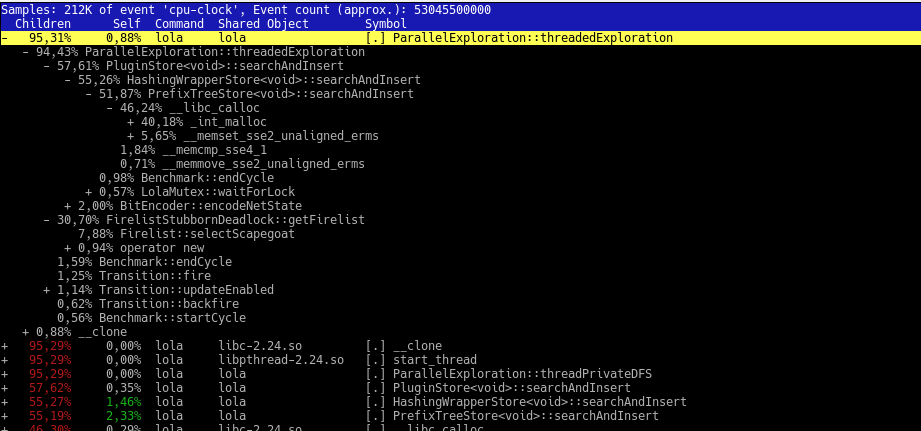
\includegraphics[width=\textwidth]{pictures/perfReportSample.png}
    \caption{perf report output}
    \label{perf_record_sample}
\end{figure}
Figure \ref{perf_record_sample} shows that over 95\% of the samples where taken somewhere in the \inline{threadedExploration}. This is expected because it is where the search of LoLA is implemented and almost all what LoLA does is searching. We can also see that nearly half of the samples where taken inside the \inline{searchAndInsert} method of the global store. This observation corresponds to the hint we took from the manual benchmark approach. The different \inline{searchAndInsert} methods are caused by the implementation of the \inline{Hashing\-Wrapper\-Store} which associate each bucket with a \inline{PrefixTreeStore} and forwards each \inline{searchAndInsert} to the corresponding \inline{PrefixTreeStore}.
The new information that we get from the data is that the most samples inside the \inline{searchAndInsert} methods are taken in a \inline{\_\_lib\_calloc} call. Almost half the samples of all taken originate here. They are almost certainly caused by allocating memory on the heap with \inline{malloc}, \inline{calloc}, or \inline{new}. This makes perfect sense, since the perpose of the \inline{searchAndInsert} method is to store newly discovered net states, which has to be done on the heap. In fact a simplified high level view on the search could be described as:
\begin{enumerate}
    \item Discover a net state
    \item Store the net state
    \item Repeat until all states are discovered
\end{enumerate}
Discovering net states is done by firing a transition from the fire list (a list of all transitions that can be fired from the current net state). Beside the \inline{searchAndInsert} method we can see this behavior in the profiling data too. Getting the fire list is the second most sampled method inside the \inline{threadedExploration} and firing the transition was also sampled often enough to account for almost 1\% of all samples.

The calls inside \inline{libcalloc} are a variety of system calls. Understanding what they really do is outside of the scope of this work. But the last sampled functions containing words like 'lock' or 'wake'. These are probably used to synchronize threads and lock memory regions. Ultimately the allocator has to be thread safe too. Allocating heap space in high frequencies is no common use case, thus the assumption that the allocator just blocks until a request was fully processed seems to be reasonable. Additionally there is only one system allocator for multiple threads. If they all call the same allocator it is likely that they get in each others ways with higher frequent calls and with an increasing amount of used threads.

With perfs data and the previous assumptions we can be quite confident that changing the way we allocate heap space can have an impact on LoLAs performance. For example we can reduce the frequent and complex calls to the allocator, by using bigger preallocated chunks of memory (from the system allocator) and manage them by our selfs. This would not only reduce the calls to \inline{libcalloc} needed, it also has the potential of reducing the overall consumed memory, since we already store pointers to each net state inside the global store. The fact that we store them permanently until LoLA is terminated makes it unnecessary to manage additional data for defragmentation handling. This information can get quite big in the system allocator, especially when allocating a lot of small data like LoLA does. The chunks can also be associated with each thread or each bucket of the \inline{Hashing\-Wrapper\-Store} to make their access thread safe. This way we can access multiple memory locations by multiple threads. If thread synchronization is really a problem by the system allocator like previously assumed, this potentially resolves the issue of the general sequential performance of LoLA with the parallel implementation.

An implementation for this approach requires a custom allocator that wraps the system calls. Fortunately we have access to exactly such an allocator from a previous project at our chair called 'mara'. The participation of the author of this work at the development of mara is another advantage. The results of this circumstances lead to an integration of mara into LoLA for the net state search.

\section{Allocation strategie change}
In the last chapter we saw that the profiling results lead deeper into the \inline{search\-And\-Insert} method. The data suggest that high frequent calls to the system allocator might be the cause of the bottleneck. To see if this assumption is true, we have to change the way LoLA uses the heap und measure the performance again.

We will use the Memory and Resource Allocator (mara) to wrap calls to the system allocator. Mara was previously developed at the chair of theoretical computer science as a student project by Julian Gaede, Marian Stein and Tom Meyer. The later use in LoLA was a part of the project goals.

A major part of maras constraints was that once allocated memory will never be rearranged and never be freed until program termination. Thus mara is allowed to drop references that where previously shared and it can be freed by the operating system. This allows mara to reduce the overhead for heap allocation in space and time.

Mara publishes a class that can be used as a custom allocator. A call to its \inline{staticNew} method will return a pointer into a previously allocated chunk of memory. The next call to \inline{staticNew} will return another pointer inside the same chunk that is adjacent to the previously returned memory segment. This memory management is equivalent to a stack. Once the chunk is filled, a new one is allocated with a call to the system allocator. The old chunk is not stored and there is no possibility to access it again with mara (but the previously shared pointers remain valid). Each object of the mara class manages disjoint parts of the heap.

With memory allocated by mara we can very easily distribute LoLAs net state memory to make it thread safe. With the \inline{Hashing\-Wrapper\-Store} we already have a method to store net states in independent \inline{PrefixTreeStore}s (inside the buckets). The access to them is already restricted to one thread at a time, while other buckets still can be accessed by other threads. This means that we do not need to consider parallelization issues inside the buckets of the \inline{PrefixTreeStore}. All memory access inside can only be done by a single thread. To use mara as allocator, we just have to create one instance of the mara class and substitute all calls to \inline{malloc}, \inline{calloc} and \inline{new} inside the \inline{PrefixTreeStore} with a call to maras \inline{staticNew} method. Because calls to delete and free will now produce undefined behavior, these calls have to be removed as well. The operating system will free the memory on program termination. After these steps, all heap allocation for the net states is wrapped by mara. 

Altering LoLA in that way we now can start another benchmark to see if the changes impact LoLAs performance. 

\begin{figure}
    \centering
    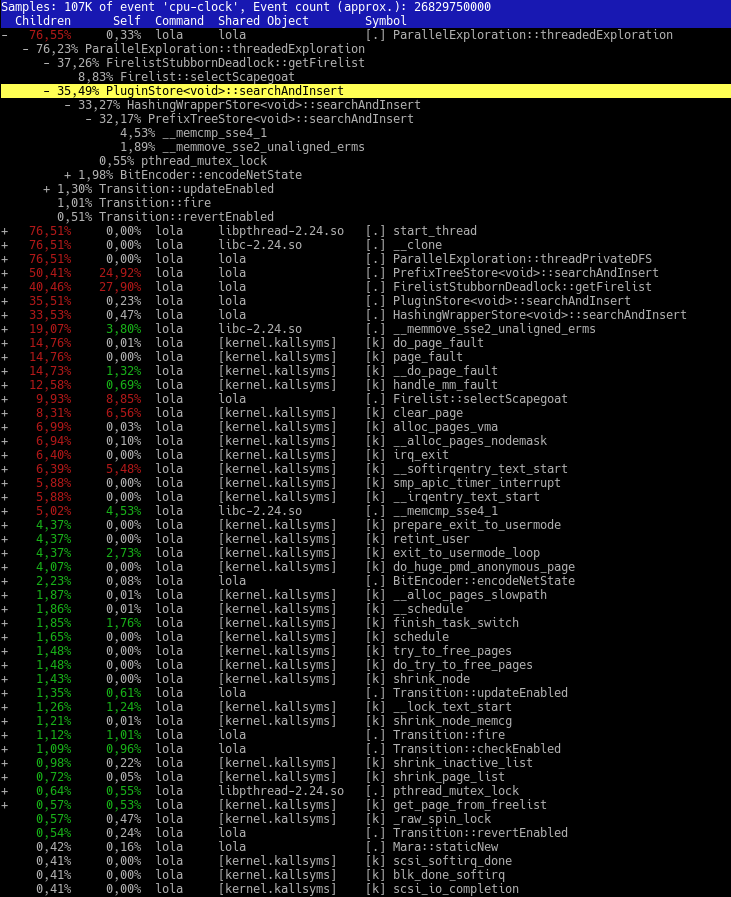
\includegraphics[width=\textwidth]{pictures/perfReportMara.png}
    \caption{perf report output of LoLA with mara integration}
    \label{perf_record_mara}
\end{figure}

\section{Results}
\subsection{Profiling}
To compare the old and the new implementation, we have to rerun our benchmark. Figure \ref{perf_record_mara} shows the output of the same mara call we used in chapter \ref{first_perf_results}.

We can see that the data changed in many ways. The \inline{searchAndInsert} and the \inline{getFirelist} methods now contribute for roughly the same amount of samples. They are also the both functions with the highest 'Self' time. This means the most samples where taken directly in this functions and not in one of their sub functions.

The most important fact however is that the calls to \inline{libcalloc} are completely gone, meaning they are under the significance threshold or where not sampled at all. Instead we can see that maras \inline{staticNew} method contributes for 0.4\% of all samples.

It seems that the integration of mara has a great impact on LoLAs performance. We seem to greatly improved the way mara uses the heap. But we do not get any information on the execution time and the thread scaling from the profiling data. To draw any conclusion we have to make additional macro benchmarks to see how the changes affects the execution time.

\subsection{Macrobenchmark}
\begin{figure}
\centering
\begin{tikzpicture}
    \begin{axis}[
        width=0.9\textwidth, 
        height=0.3\textheight,
        xbar, axis on top,
        xmajorgrids=true,
        bar width=16,
        title={Macro Benchmark},
        xtick={0,50,100,150,200,250,300},
        xmin=0,
        x tick label style={/pgf/number format/1000 sep=},
        xlabel={seconds},
        ytick={1,2,3,4},
        yticklabels={PThread,CAS,Mara Pthread,Mara CAS},
        y tick label style={/pgf/number format/1000 sep=},
        bar shift=0,
        enlarge y limits=0.5,
        nodes near coords,
        nodes near coords align={horizontal},
        %
        legend style={
            at={(0.5,-0.15)},
            anchor=north,
            legend columns=2,
            /tikz/every even column/.append style={column sep=0.5cm}
        }
        ]
        \legend{PThread, Compare And Swap, Mara Pthread, Mara Compare And Swap}

        \addplot table [x=master-t1-b0, y expr=1, col sep=comma,trim cells=true] {data/allMacroData.csv};
        \addplot table [x=atomics-t1-b0, y expr=2, col sep=comma,trim cells=true] {data/allMacroData.csv};
        \addplot table [x=maraPThread-t1-b0, y expr=3, col sep=comma,trim cells=true] {data/allMacroData.csv};
        \addplot table [x=maraIntegration-t1-b0, y expr=4, col sep=comma,trim cells=true] {data/allMacroData.csv};
    \end{axis}
\end{tikzpicture}
\caption{Macro benchmark comparison between the original (PThread) implementation and the substitute (Compare and swap)\\ LoLA call: "lola --check=full --threads=4 ../tests/testfiles/phils1000.lola" }
\end{figure}
There are different questions that are of interest with the new implementation. To address a variety of them multiple tests were issued. We can divide them into three categories:
\begin{enumerate}
    \item Single thread performance,
    \item Implementation comparison and
    \item Bucket influence.
\end{enumerate}
The single thread performance will be compared without the use of the \inline{Hashing\-Wrapper\-Store}. This way we can observe any efficiency difference that are caused by mara or the compare and swap (CAS) synchronization.
To have insight into the thread scaling we will compare all implementations with use of the \inline{Hashing\-Wrapper\-Store} combined with a different amount of threads.
And to see how the amount of used buckets influences the results, we will look at the implementations that are scaling with the threads.

We will investigate all implementation changes. The preexisting unchanged implementation will be called 'PThread', The implementation with the changed synchronization method will be called 'CAS' and implementation with the integration of mara will be called 'Mara PThread'. Additionally we will look at an implementation where the CAS synchronization and the mara integration was used. It will be called 'Mara CAS'.

In this case we will run the benchmarks on ebro because it can access up to 64 threads. However we will limit the thread count to a maximum of 50 so that other tasks are unlikely to interfere with our benchmark.

%TODO: check if this statement is true
The benchmark values will be an average of 10 runs, so that performance deviations are compensated.

In the single thread benchmark - shown in figure \ref{SingleThreadBenchmark} - a quite homogeneous characteristic can be observed. The difference between the CAS and the Pthread implementation is insignificant. But we can observe a speedup between the mara and non mara implementations. With a single thread the pthread mutexes seem to work slightly faster than the compare and swap approach.

\begin{figure}
    \centering
    \begin{tikzpicture}
        \begin{axis}[
            width=0.9\textwidth, 
            height=0.95\textheight,
            xbar=-11.5, axis on top,
            xbar legend,
            xmajorgrids=true,
            bar width=14,
            title={Macro Benchmark},
            xmin=0,
            x tick label style={/pgf/number format/1000 sep=},
            xlabel={seconds},
            ymin=1,
            ymax=6,
            ylabel={thread count},
            ytick={1,2,3,4,5,6},
            yticklabels={1,2,3,4,20,50},
            y tick label style={/pgf/number format/1000 sep=},
            enlarge y limits=0.12,
            nodes near coords,
            nodes near coords align={horizontal},
            %
            legend entries={PThread,,,,,,CAS,,,,,,Mara CAS,,,,,,Mara Pthread},
            legend style={
                at={(0.98,0.02)},
                anchor=south east,
            %     legend columns=2,
            %     /tikz/every even column/.append style={column sep=0.5cm}
            } 
            ]

        \addplot [blue, fill=blue!30] table [x=master-t1-b100, y expr=1, col sep=comma,trim cells=true] {data/allMacroData.csv};
        \addplot [blue, fill=blue!30] table [x=master-t2-b100, y expr=2, col sep=comma,trim cells=true] {data/allMacroData.csv};
        \addplot [blue, fill=blue!30] table [x=master-t3-b100, y expr=3, col sep=comma,trim cells=true] {data/allMacroData.csv};
        \addplot [blue, fill=blue!30] table [x=master-t4-b100, y expr=4, col sep=comma,trim cells=true] {data/allMacroData.csv};
        \addplot [blue, fill=blue!30] table [x=master-t20-b100, y expr=5, col sep=comma,trim cells=true] {data/allMacroData.csv};
        \addplot [blue, fill=blue!30] table [x=master-t50-b100, y expr=6, col sep=comma,trim cells=true] {data/allMacroData.csv};

        \addplot [red, fill=red!30] table [x=atomics-t1-b100, y expr=1, col sep=comma,trim cells=true] {data/allMacroData.csv};
        \addplot [red, fill=red!30] table [x=atomics-t2-b100, y expr=2, col sep=comma,trim cells=true] {data/allMacroData.csv};
        \addplot [red, fill=red!30] table [x=atomics-t3-b100, y expr=3, col sep=comma,trim cells=true] {data/allMacroData.csv};
        \addplot [red, fill=red!30] table [x=atomics-t4-b100, y expr=4, col sep=comma,trim cells=true] {data/allMacroData.csv};
        \addplot [red, fill=red!30] table [x=atomics-t20-b100, y expr=5, col sep=comma,trim cells=true] {data/allMacroData.csv};
        \addplot [red, fill=red!30] table [x=atomics-t50-b100, y expr=6, col sep=comma,trim cells=true] {data/allMacroData.csv};

        \addplot [green, fill=green!30] table [x=maraIntegration-t1-b100, y expr=1, col sep=comma,trim cells=true] {data/allMacroData.csv};
        \addplot [green, fill=green!30] table [x=maraIntegration-t2-b100, y expr=2, col sep=comma,trim cells=true] {data/allMacroData.csv};
        \addplot [green, fill=green!30] table [x=maraIntegration-t3-b100, y expr=3, col sep=comma,trim cells=true] {data/allMacroData.csv};
        \addplot [green, fill=green!30] table [x=maraIntegration-t4-b100, y expr=4, col sep=comma,trim cells=true] {data/allMacroData.csv};
        \addplot [green, fill=green!30] table [x=maraIntegration-t20-b100, y expr=5, col sep=comma,trim cells=true] {data/allMacroData.csv};
        \addplot [green, fill=green!30] table [x=maraIntegration-t50-b100, y expr=6, col sep=comma,trim cells=true] {data/allMacroData.csv};

        \addplot [orange, fill=orange!30] table [x=maraPThread-t1-b100, y expr=1, col sep=comma,trim cells=true] {data/allMacroData.csv};
        \addplot [orange, fill=orange!30] table [x=maraPThread-t2-b100, y expr=2, col sep=comma,trim cells=true] {data/allMacroData.csv};
        \addplot [orange, fill=orange!30] table [x=maraPThread-t3-b100, y expr=3, col sep=comma,trim cells=true] {data/allMacroData.csv};
        \addplot [orange, fill=orange!30] table [x=maraPThread-t4-b100, y expr=4, col sep=comma,trim cells=true] {data/allMacroData.csv};
        \addplot [orange, fill=orange!30] table [x=maraPThread-t20-b100, y expr=5, col sep=comma,trim cells=true] {data/allMacroData.csv};
        \addplot [orange, fill=orange!30] table [x=maraPThread-t50-b100, y expr=6, col sep=comma,trim cells=true] {data/allMacroData.csv};
    \end{axis}
\end{tikzpicture}
%TODO:Caption ändern
\caption{Macro benchmark comparison between the original (PThread) implementation and the substitute (Compare and swap)\\ LoLA call: "lola --check=full --threads=4 ../tests/testfiles/phils1000.lola" }
\end{figure}
The benchmark for the implementation comparison shows that the original implementation is quite consistent between the used threads. This is due to bugs that will be explained in chapter \ref{evaluation}. We can see again that the CAS implementation nether really outperforms the original implementation but with the addition that at a very high thread count the execution time rises again to very high levels. The both mara implementation however are able to outperform the PThread implementation at a certain thread count, even though they are performing considerably worse on a lower thread count.

\begin{figure}
\centering
\begin{tikzpicture}
    \begin{axis}[
        width=0.9\textwidth, 
        height=0.95\textheight,
        xbar=-11.5, axis on top,
        xbar legend,
        xmajorgrids=true,
        bar width=14,
        title={Macro Benchmark},
        xmin=0,
        x tick label style={/pgf/number format/1000 sep=},
        xlabel={seconds},
        ymin=1,
        ymax=6,
        ylabel={thread count},
        ytick={1,2,3,4,5,6},
        yticklabels={1,2,3,4,20,50},
        y tick label style={/pgf/number format/1000 sep=},
        enlarge y limits=0.12,
        nodes near coords,
        nodes near coords align={horizontal},
        %
        legend entries={Mara CAS 100 buckets,,,,,,Mara Pthread 100 buckets,,,,,,Mara CAS 1000 buckets,,,,,,Mara Pthread 1000 buckets},
        % legend style={
        %     at={(0.5,-0.1)},
        %     anchor=north,
        %     legend columns=2,
        %     /tikz/every even column/.append style={column sep=0.5cm}
        % } 
        ]

        \addplot [blue, fill=blue!30] table [x=maraIntegration-t1-b100, y expr=1, col sep=comma,trim cells=true] {data/allMacroData.csv};
        \addplot [blue, fill=blue!30] table [x=maraIntegration-t2-b100, y expr=2, col sep=comma,trim cells=true] {data/allMacroData.csv};
        \addplot [blue, fill=blue!30] table [x=maraIntegration-t3-b100, y expr=3, col sep=comma,trim cells=true] {data/allMacroData.csv};
        \addplot [blue, fill=blue!30] table [x=maraIntegration-t4-b100, y expr=4, col sep=comma,trim cells=true] {data/allMacroData.csv};
        \addplot [blue, fill=blue!30] table [x=maraIntegration-t20-b100, y expr=5, col sep=comma,trim cells=true] {data/allMacroData.csv};
        \addplot [blue, fill=blue!30] table [x=maraIntegration-t50-b100, y expr=6, col sep=comma,trim cells=true] {data/allMacroData.csv};

        \addplot [red, fill=red!30] table [x=maraPThread-t1-b100, y expr=1, col sep=comma,trim cells=true] {data/allMacroData.csv};
        \addplot [red, fill=red!30] table [x=maraPThread-t2-b100, y expr=2, col sep=comma,trim cells=true] {data/allMacroData.csv};
        \addplot [red, fill=red!30] table [x=maraPThread-t3-b100, y expr=3, col sep=comma,trim cells=true] {data/allMacroData.csv};
        \addplot [red, fill=red!30] table [x=maraPThread-t4-b100, y expr=4, col sep=comma,trim cells=true] {data/allMacroData.csv};
        \addplot [red, fill=red!30] table [x=maraPThread-t20-b100, y expr=5, col sep=comma,trim cells=true] {data/allMacroData.csv};
        \addplot [red, fill=red!30] table [x=maraPThread-t50-b100, y expr=6, col sep=comma,trim cells=true] {data/allMacroData.csv};

        \addplot [green, fill=green!30] table [x=maraIntegration-t1-b1000, y expr=1, col sep=comma,trim cells=true] {data/allMacroData.csv};
        \addplot [green, fill=green!30] table [x=maraIntegration-t2-b1000, y expr=2, col sep=comma,trim cells=true] {data/allMacroData.csv};
        \addplot [green, fill=green!30] table [x=maraIntegration-t3-b1000, y expr=3, col sep=comma,trim cells=true] {data/allMacroData.csv};
        \addplot [green, fill=green!30] table [x=maraIntegration-t4-b100, y expr=4, col sep=comma,trim cells=true] {data/allMacroData.csv};
        \addplot [green, fill=green!30] table [x=maraIntegration-t20-b1000, y expr=5, col sep=comma,trim cells=true] {data/allMacroData.csv};
        \addplot [green, fill=green!30] table [x=maraIntegration-t50-b1000, y expr=6, col sep=comma,trim cells=true] {data/allMacroData.csv};

        \addplot [orange, fill=orange!30] table [x=maraPThread-t1-b1000, y expr=1, col sep=comma,trim cells=true] {data/allMacroData.csv};
        \addplot [orange, fill=orange!30] table [x=maraPThread-t2-b1000, y expr=2, col sep=comma,trim cells=true] {data/allMacroData.csv};
        \addplot [orange, fill=orange!30] table [x=maraPThread-t3-b1000, y expr=3, col sep=comma,trim cells=true] {data/allMacroData.csv};
        \addplot [orange, fill=orange!30] table [x=maraPThread-t4-b1000, y expr=4, col sep=comma,trim cells=true] {data/allMacroData.csv};
        \addplot [orange, fill=orange!30] table [x=maraPThread-t20-b1000, y expr=5, col sep=comma,trim cells=true] {data/allMacroData.csv};
        \addplot [orange, fill=orange!30] table [x=maraPThread-t50-b1000, y expr=6, col sep=comma,trim cells=true] {data/allMacroData.csv};
    \end{axis}
\end{tikzpicture}
%TODO:Caption ändern
\caption{Macro benchmark comparison between the original (PThread) implementation and the substitute (Compare and swap)\\ LoLA call: "lola --check=full --threads=4 ../tests/testfiles/phils1000.lola" }
\end{figure}
But to utilize a maximum of the parallelization capabilities, the memory has to be used efficiently. Increasing the amount of threads will increase the probability of concurrent access of the same bucket. In this case the bucket will grant access to a single thread and will lock the execution of the others. Thus a higher thread count will ultimately a again decreasing performance at least of a single thread.

We can can decrease the chances of concurrent access by increasing the amount of used buckets. Therefore figure \ref{MaraBucketComparison} shows the performance of the mara implementations with a different amount of buckets. We can observe a general performance gain with a higher amount of buckets. Even single threaded. The difference slowly diminishes with more threads. However, a greater bucket count preserves a better thread scaling. We can se a further decreasing of the execution time with more buckets on a higher thread count, whereas the execution time of CAS with 100 buckets increases again between 20 and 50 used threads.

At this point we can summerize that we have affected the performance with the new implementations. In some cases even for the better. In the next chapter we will evaluate the data in more detail.

\subsection{Evaluation}
\label{evaluation}
We saw that the new implementations perform differently in the results of the benchmark. We can now analyze what the causes for these differences are.

But before that it should be stated again that the benchmarks where run on a single petri net and on a single machine. While the used hardware should hardly influence the relative performance differences, the test data can have a major effect. For example a petri net, where always at most on transition is fireable in each state, can not be searched in parallel by the current algorithm. In such a case we would see no benefit by using multiple threads and parallelization would certainly perform worse due to its synchronization overhead.

Additionally the use of LoLA with the \inline{--check=full} parameter is by far not the only possible use of LoLA. It is probably most used with a predicate to check. In that case, the petri net is often reduced to a smaller (in respect to the predicate) äquivalent net, before the search is done. This again can influence the number of fireable transistions and therefore the potential of the parallel search.

That said, the following should be seen as a constrictive comparison between the sequential and parallel capabilities of LoLA not as an exhaustive one.

\subsubsection{Single thread performance}
\label{evalSingleThread}
We have two different results on the single thread performance of LoLA. If the \inline{Hashing\-Wrapper\-Store} is used all new implementations perform worse than the initial implementation. If it is not used the mara implementations perform better.

The performance gain in the latter can be explained exactly by the use of mara. Benchmarks in the development of mara showed that it is faster than a call to \inline{malloc}, because it can reduce an allocation call to basically three stack operations:
\begin{enumerate}
    \item Save the current stack pointer
    \item Increase the stack pointer by the size of the requested data
    \item Return the saved pointer
\end{enumerate}
Because LoLA requests a lot of heap space, this adds up to a significant amount of time.

But when we introduce the \inline{Hashing\-Wrapper\-Store} with its buckets, the performance of all new implementations drop considerably, while the initial implementation gains performance. 

The performance gain can be explained by the concept of the \inline{Hashing\-Wrapper\-Store}. When we distribute all states evenly between the buckets, we can do an informed search later because we know the bucket associated with our hash value. Since every insert of a net state implies a previous search to avoid duplicates, it is possible to reduce the execution time with a suitable amount of buckets.

The performance loss can be explained by the implementation of the \inline{Hashing\-Wrapper\-Store}. The original implementation was not guarded by mutexes and therefore not thread safe. Additionally the bucket count from the lola call was ignored and a hard coded value was used instead. This suggest that the implementation was incomplete and the use of buckets was experimental. For the use in the new implementations, the \inline{Hashing\-Wrapper\-Store} had to be altered. Now, before a bucket will be accessed via hash, a mutex has to be passed to prevent concurrent access and a modulo check is done to assure that a bucket to insert exists. These new operations can accumulate to a lot of time with frequent use by LoLA.

However, asside from the synchronization issues it seems that mara has the potential to speed up the execution in general. The heap allocation is independent from the depth first search and the optimization techniques incorporated by LoLA. 

Also it might be possible to affect the memory space consumption with mara. Though not benchmarked explicitly, while testing the implementations during development, a considerable memory reduction was observed. While the 1000 philosophers caused a premature termination of the tests with the \inline{Hashing\-Wrapper\-Store}, the mara integration enabled LoLA to finish the test successful under the right circumstances. With the approximately 17GB of RAM on the VM, the original implementation terminated at about the half of net states to discover. But with a chunk size of 500MB it was possible to fit all net states in the memory. It can be assumed that this is a saving of multiple giga bytes and might be a matter that is worth investigating more in depth.

To address the worse performance with the changes in the \inline{Hashing\-Wrapper\-Store}, it might be possible to reduce the execution time by checking with how many threads LoLA runs. A condition to skip the mutexe blocks when using only one thread or a completely new class that is loaded dynamically single threaded can be implemented. Anyway, the performance gap between the hashed and unhashed execution of the PThread implementation suggest that this matter can buy in execution time at expense for memory space.

\subsubsection{Thread scaling}
The main goal of this work was to achieve a scaling with the threads. As we can see from the benchmark data, the initial PThread implementation is not affected by the number of threads at all. The reason for this is that - due to a bug - the configured thread count is completely ignored. 

The bug is caused by a differing function signatures. LoLA uses different class for the depth first search when using one thread and when using more than one thread. If LoLA is initialized with one thread it uses the \inline{DFSExploration} class and with more threads it uses the \inline{ParallelExploration} class (that is derived from the DFSExploration). To start the search the \inline{depth\_first} method is called with the signature '\inline{bool depth\_first SimpleProperty, NetState, Store<void>, Firelist, int)}'. This method is implemented in the \inline{DFSExploration} class. But in the \inline{ParallelExploration} class a method with the signature '\inline{bool depth\_first SimpleProperty, NetState, Store<void>, Firelist, threadid\_t)}' is implemented. This probably causes an additional entry in the objects virtual table so that the \inline{depth\_first} method appears multiple times with the two different signatures. Since LoLA calls the search method in the \inline{ParallelExploration} with the first signature the (sequential) base implementation is used instead of the new one. The bug is fixed simply by changing the child signatures \inline{threadid\_t} to an \inline{int}.

If this bug is resolved we can observe an increasing performance with an increasing amount of threads. At least in the lower range. With 50 threads the CAS implementation performs worst. Since the test was run with 100 buckets, this behavior can be explained with an increased blocking of threads not only on entering a bucket, but also on allocating heap memory with \inline{calloc}. The latter seems to have a greater effect if we compare the results with the mara implementations.

After switching to mara, the allocator blocking seems to be gone as expected. The mara implementations are the first to beat the single threaded implementation with a high amount of threads. This leads to the assumption that allocating heap space with the system allocator was the main cause of the previous bottleneck. We can even see a linear scaling in the range from two to four threads. The performance does not split in half from one to two threads, because the single threaded algorithm does use the original \inline{DFSExploration} which comes with much less synchronization overhead.

In contrast to the first impression it is even possible that the linear scaling reaches the higher thread range. Eventually LoLA has a single threaded build up and tear down phase. This phases are included in LoLAs internal measurement and therefore are included in the results. But since we do not have reliable data for that phases, this matter will remain speculative for now.

\subsubsection{Bucket influence}
We can see continuous improvement with the use of additional buckets in the mara implementations. 

One reason for that is probably the decreased chance for concurrent access. This gets more important with increasing threads. In fact we can see a slight decrease of the mara CAS performance between 20 and 50 threads that seems to be compensated with the use of more buckets.

But the increasing single thread performance cannot be explained by less bucket conflicts. Like described in \ref{evalSingleThread}, this behavior is probably caused by a reduced store search time. Because LoLA distributes all states in the buckets and knows in which bucket to search for a given net state, the overall search time is decreasing.

However, the extend of both effects is not reflected in the data. To evaluate this matter a macro benchmark does not suffice.
